\documentclass[a4paper, notitlepage, 10pt]{report}
\usepackage[italian]{babel}
\usepackage[T1]{fontenc}
\usepackage[utf8]{inputenc}
\usepackage{amsmath}
\usepackage{amsfonts}
\usepackage{amsthm}
\usepackage{frontespizio}
\usepackage{hyperref}
\hypersetup{hidelinks,
	colorlinks = true,
	urlcolor = black, 
	linkcolor = black}
\usepackage[margin=3cm]{geometry}
\usepackage{booktabs}
\usepackage{fancyhdr}
\usepackage{listings}
\usepackage{stmaryrd}
\usepackage[strict]{changepage}
\usepackage{galois}
\usepackage{libertine}
\usepackage{textcomp}
\usepackage{float}
\usepackage{multicol}
\usepackage{makecell}
\usepackage{stmaryrd}
\usepackage{amssymb}
\usepackage{caption}
\renewcommand\theadalign{bc}
\renewcommand\theadfont{\bfseries}
\renewcommand\theadgape{\Gape[4pt]}
\renewcommand\cellgape{\Gape[4pt]}

\lstset{basicstyle=\ttfamily\small}

\newtheorem{definit}{Definizione}[subsection]
\newtheorem{thm}{Teorema}[subsection]


\makeatletter
\newcommand*{\toccontents}{\@starttoc{toc}}
\makeatother

\begin{document}
	\title{\textbf{\underline{Sistemi a Eventi Discreti}}}
	\date{Febbraio 2018}
	\author{Colognese, Rossini}
	\maketitle
	
	\toccontents

\chapter*{Concetti di Base}
\addcontentsline{toc}{chapter}{Concetti di Base}

\subsection*{Composizione parallela: $H || G$}
\addcontentsline{toc}{section}{Composizione parallela: $H || G$}
\begin{itemize}
	\item Si crea uno stato iniziale composto dagli stati iniziali dei due grafi;
	\item si effettua una transizione di uno dei grafi, modificando la nuova coppia di stati, ad esempio:
	\begin{itemize}
		\item nel grafo G, il nodo A va in B con la transizione $a_1$;
		\item nel grafo H, se con $a_1$ il nodo 1 va in 2, allora il nuovo stato è $(B, 2)$;
		\item nel grafo H, se con $a_1$ il nodo 1 non ha mosse disponibili, allora il nuovo stato è $(B, 1)$;
	\end{itemize}
	\item effettuare tutte le transizioni di entrambi i grafi generando tutte le combinazioni possibili.
	
	Per alcuni eventi, bisogna tenere conto della specifica dell'esercizio ($H_{spec} ~||~ G$).
\end{itemize}

\subsection*{Prodotto: $H \times G$}
\addcontentsline{toc}{section}{Prodotto: $H \times G$}
\begin{itemize}
	\item Si crea uno stato iniziale composto dagli stati iniziali dei due grafi;
	\item si effettua una transizione, modificando la nuova coppia di stati, verificando che entrambi possano eseguirla. Ad esempio, se nel grafo G, il nodo A va in B con la transizione $a_1$:
	\begin{itemize}
		\item se nel grafo H il nodo 1 va in 2 con $a_1$, allora il nuovo stato è $(B, 2)$;
		\item se il grafo H non ha mosse disponibili con $a_1$ dal nodo 1, la transizione viene saltata;
	\end{itemize}
	\item effettuare tutte le transizioni di entrambi i grafi generando tutte le combinazioni possibili.
\end{itemize}

\subsection*{Coaccessibilità: $CoAcc (G)$}
\addcontentsline{toc}{section}{Coaccessibilità: $CoAcc (G)$}
Elimina tutti gli stati che andranno solamente in stati di \textit{deadlock} oppure \textit{livelock}.

\subsection*{Accessibilità: $Acc (G) = Trim(G)$}
\addcontentsline{toc}{section}{Accessibilità: $Acc (G) = Trim(G)$}
Elimina tutti gli stati che non possono essere raggiunti da $S_0$ attraverso una o più transizioni.

\subsection*{Complemento: $Compl (G)$}
\addcontentsline{toc}{section}{Complemento: $Compl (G)$}
Si convertono tutti gli stati non-terminali in stati terminali e viceversa. Si aggiungono inoltre tutte le transizioni mancanti per completare l'alfabeto del linguaggio; se necessario si aggiunge uno stato accettante (terminale) per le transizioni mancanti.



\chapter*{Linguaggi e Automi}
\addcontentsline{toc}{chapter}{Linguaggi e Automi}

\section*{Osservatore}
\addcontentsline{toc}{section}{Osservatore}
Considerando un automa (possibilmente non deterministico) $G_{nd} = (X, E ~\cup~ \{\epsilon \}, f_{nd}, \gamma, x_0, X_m)$, l'insieme degli eventi $E = E_o ~\cup~ E_{uo}$ è così suddiviso:
\begin{itemize}
	\item $E_{o}$ : insieme degli eventi osservabili;
	\item $E_{uo}$ : insieme degli eventi non osservabili (comprende le $\epsilon$-transizioni).
\end{itemize}

Per costruire l'osservatore per il grafo $G$, si seguono i seguenti passi:
\begin{itemize}
	\item sostituire con $\epsilon$ tutte le transizioni corrispondenti a eventi non osservabili;
	\item convertire l'automa NFA in DFA:
	\begin{itemize}
		\item si prende lo stato iniziale e si crea uno stato includendo anche gli stati raggiungibili con $\epsilon$-transizioni;
		\item per ogni altra transizione $t$ si creano gruppi di stati raggiungibili con $t$ e con $\epsilon$;
		\item lo stato che contiene $S_f$ di G sarà lo stato finale dell'osservatore.
		\end{itemize}
\end{itemize}



\section*{Osservabilità}
\addcontentsline{toc}{section}{Osservabilità}
Per verificare l'osservabilità di un sistema:
\begin{itemize}
	\item costruire il grafo corrispondente al linguaggio marcato;
	\item riscriverlo disabilitando gli archi con transizione controllabile uscente dallo stato iniziale (lasciare gli incontrollabili);
	\item costruire osservatore sostituendo le transizioni non osservabili con $\epsilon$:
	\begin{itemize}
		\item se uno stato non terminale (composto da più stati) ha una transizione controllabile che è stata disabilitata per uno dei suoi componenti, allora il sistema \textit{non è osservabile};
		\item se viene disabilitata per un componente dello stato finale allora il sistema \textit{è osservabile}.
	\end{itemize}
\end{itemize}
\noindent
Si considerino i linguaggi $K$ e $M = \overline{M}$ definiti sull'alfabeto di eventi $E$, con $E_c \subseteq E$, $E_o \subseteq E$ e $P$ la proiezione naturale da $E* \Rightarrow E_0*$.
\\$K$ è osservabile rispetto a $M$, $E_o$, $E_c$ se per tutte le stringhe $s \in \overline{K}$ e per tutti gli eventi $\sigma \in E_c$ si ha: 
$$(s\sigma \notin \overline{K}) \land (s\sigma \in M) \Rightarrow P^{-1}[P(s)] \sigma  \cap \overline{K} = \emptyset$$
L'insieme di stringhe denotato dal termine $P^{-1}[P(s)] \sigma \cap \overline{K}$ contiene tutte le stringhe che hanno la medesima proiezione di $s$ e possono essere prolungate in $K$ con il simbolo $\sigma$. Se tale insieme non è vuoto, allora $K$ contiene due stringhe $s$ e $s'$ tali che $P(s)=P(s')$ per cui s$\sigma \notin \overline{K}$ e $s'\sigma \in \overline{K}$. Un supervisore non saprebbe distinguere tra $s$ e $s'$ per l'osservabilità. Non potrebbe quindi esistere un supervisore che ottiene esattamente il linguaggio $\overline{K}$.

La proiezione va fatta sul linguaggio (prefissi).
\\

$P^{-1}[P(\epsilon)] = P^{-1}[\epsilon] = \{e^*\}$, con $e\in E_{uo}$.

$P(aaa) = \{aaa\}$, ad esempio con $E=\{a, b\}$.

$P^{-1}[P(aa)] = \{aa, bb, ab, ba \}$, se $a$ e $b$ sono eventi indistinguibili con $E=\{a, b\}$.


\section*{Controllabilità}
\addcontentsline{toc}{section}{Controllabilità}
Un linguaggio può essere controllabile (esiste una strategia di controllo) anche se non è realizzabile da un automa a stati finiti (es. $K = \{a^n b^m$ con $n\geq m\geq 0\}$).
\\\\
Per verificare la controllabilità di un sistema:
\begin{itemize}
	\item l'evento incontrollabile non può essere disabilitato, quindi disabilitare quello controllabile;
	\item dopo che l'impianto ha prodotto l'evento incontrollabile si riabilita l'evento controllabile.
\end{itemize}
Se la stringa prodotta corrisponde a quella voluta $K$ allora \textit{è controllabile}.
\\
Cioè è controllabile solo se l'evento incontrollabile è il primo evento dalla stringa $K$.
\\
\\
Si prende una stringa $s \in \overline{K}$, si prende poi una stringa $\sigma \in E_{uc}$. Se la concatenazione $s\sigma \in M \in \overline{K}$ allora il sistema è controllabile. Se invece $s\sigma \in M \notin \overline{K}$ allora non è controllabile ($\overline{K} = L(H) ~\text{e}~ H = H_{spec} || G$).



\section*{Controllore Massimo Supremo}
\addcontentsline{toc}{section}{Controllore Massimo Supremo}
Controllore massimo supremo: $K^{\uparrow C} = L(H)^{\uparrow C}$.
\\
Per $K=\overline{K}$ abbiamo: $K^{\uparrow C} = K\backslash [M\backslash K / E^*_{uc}] E^*$.
\\
Dati $G_1$ e $G_2$:
\begin{itemize}
	\item costruire $G = G_1 || G_2$, $M = L(G)$;
	\item costruire $H_{spec}$ seguendo le specifiche e individuare $L(H_{spec})$;
	\item costruire $H = H_{spec} || G$ tenendo conto della specifica ($K = L(H)$);
	\item verificare la controllabilità con $s\sigma \in M \in \overline{K}$;
	\item costruire $H_0 = H \times G$ assumendo $\mathcal{L}_m(H_0) = K$ e $\mathcal{L}(H_0) = \overline{K}$;
	\item calcolare $K^{\uparrow C}$ con il seguente algoritmo:
	\begin{itemize}
		\item rimuovere per incontrollabilità da $H_0$ i nodi composti che non hanno l'arco uscente con evento non controllabile perché uno dei due nodi che lo compongono non ha l'uscita corrispondente;
		\item rimuovere per potatura gli stati non terminali che non vanno in uno stato marcato;
		\item se la precedente eliminazione causa la perdita di archi con evento non controllabile, ripetere l'algoritmo.
	\end{itemize}
\end{itemize} 
\noindent
L'automa ottenuto (anche vuoto) sarà il Controllore Massimo Supremo.

\section*{Sovralinguaggio Controllabile Infimo}
\addcontentsline{toc}{section}{Sovralinguaggio Controllabile Infimo}
Sovralinguaggio controllabile infimo chiuso rispetto al prefisso: $K^{\downarrow C} = \overline{K} E^*_{uc} \cap M$.
\\
Dati $G_1$ e $G_2$:
\begin{itemize}
	\item costruire $G = G_1 || G_2$, $M = L(G)$;
	\item costruire $H_{spec}$ seguendo le specifiche e individuare $L(H_{spec})$;
	\item costruire $H = H_{spec} || G$ tenendo conto della specifica ($K = L(H)$);
	\item calcolare $K^{\downarrow C}$ con il seguente algoritmo:
	\begin{itemize}
		\item aggiungere un nodo $N$ avente un auto-anello con gli eventi non controllabili e collegare tutti gli altri nodi a $N$ con $\epsilon$ transizioni;
		\item $\forall$ nodo sostituire $\epsilon$ con l'evento/i non controllabile a esso mancante, ottenendo così $H_{aug}$;
		\item costruire l'automa $H_{aug} \times G$ ottenendo $K^{\downarrow C}$.
	\end{itemize}
\end{itemize}


\chapter*{Segnali discreti}
\addcontentsline{toc}{chapter}{Segnali discreti}
Se $T \subseteq R$ e’ l’insieme dei tempi in cui $e$ è presente, cioè $T = \{t \in R : e(t) \neq assente\}$, il segnale $e$ è discreto se esiste una funzione iniettiva $f : T \rightarrow N$ che preserva l’ordine, cioè $\forall t_1, t_2 \in T$ se $t_1 \leq t_2$ allora $f(t_1) \leq f(t_2)$. L’esistenza di tale funzione iniettiva garantisce che possiamo contare gli eventi secondo un ordine temporale.

Un segnale è discreto se:
\begin{itemize}
	\item riesco a metterlo in corrispondenza dei numeri naturali;
	\item è definito sugli interi non negativi: basta prendere come $f$ la funzione identità che è iniettiva e preserva banalmente l’ordine;
	\item non è definito sui razionali: i tempi in cui è presente non possono essere contati in ordine (essi non sono una successione di eventi istantanei nel tempo, bensì un insieme di eventi istantanei nel tempo);
	\item se $t = 1 - \frac{1}{n}$ per ogni intero positivo $n$: poiché in questo caso l’insieme dei tempi in cui il segnale $y$ è presente è $T = \{1-\frac{1}{1},1-\frac{1}{2},1-\frac{1}{3},...,1-\frac{1}{n},...\}= \{0, \frac{1}{2}, \frac{2}{3}, . . . \}$ possiamo definire $f$ come $\forall t\in T : f(t)=n$, dove $t=1-\frac{1}{n}$ che è iniettiva e preserva l’ordine;
	\item non è combinazione di due segnali di cui almeno uno non è discreto.
\end{itemize}

\noindent
Se due segnali sono discreti, la loro combinazione può non esserlo: $x(n)$ e $y(1 - \frac{1}{n})$ con $n\in \mathbb{Z}$.

{\let\clearpage\relax \chapter*{Reti di Petri}}
\addcontentsline{toc}{chapter}{Reti di Petri}


\subsection*{Albero di Copertura (o Raggiungibilità)}
\addcontentsline{toc}{section}{Albero di Copertura (o Raggiungibilità)}
Dato una marcatura iniziale si effettuano tutte le possibili transizioni ottenendo nuove marcature.
L'albero si conclude quando non è possibile effettuare altre transizioni oppure quando si ottengono marcature già trovate (\textit{dup}).
\\
Se un nodo $y$ è già presente nell'albero e il nuovo nodo $x$ copre quello vecchio (e c'è un percorso da $y$ a $x$), allora si mette $x(p)=\omega$ per ogni $p$ avente $x'(p)>y(p)$.
\\\\
Dall'albero si può ricavare il linguaggio della Rete di Petri (ogni transizione corrisponde ad un carattere).


\subsection*{Grafo di Copertura (o Raggiungibilità)}
\addcontentsline{toc}{section}{Grafo di Copertura (o Raggiungibilità)}
Dato un albero di copertura si sostituiscono i \textit{dup} con archi all'indietro.
\\\\
\textit{\textbf{Grafo Marcato}}: rete in cui ogni posto ha esattamente un arco in ingresso e uno in uscita.
\\
\textit{\textbf{Reti a Scelta Libera}}: rete in cui ogni arco da $p$ a $t$, o è l'unico uscente da $p$ o è l'unico entrante in $t$.



\chapter*{Macchine a stati}
\addcontentsline{toc}{chapter}{Macchine a stati}
\textit{\textbf{Macchina a Stati}}: è una rete di Petri in cui ogni transizione ha un arco in ingresso e uno in uscita.\\
Le reti di Petri sono più espressive degli automi a stati finiti. Esse corrispondono ad automi a stati finiti quando hanno un numero finito di marcature raggiungibili (rete di Petri limitata).
\\\\
Date le tracce degli ingressi/uscite costruire:
\begin{itemize}
	\item \textit{Grafo di Transizione dei Segnali (STG)}: grafo con input e output seguiti da +/- e collegati tra loro. È un modello per diagrammi temporali. È una rete di Petri interpretata dove le transizioni sono rappresentate dalle loro etichette e si omettono i posti. I gettoni indicano lo stato iniziale del sistema;
	\item \textit{Reti di Petri}: questi diventano transizioni e tra una transizione e l'altra si inseriscono i posti, inserire anche i token nei posti precedenti alle prime transizioni;
	\item \textit{Grafo di Raggiungibilità}: fare tutte le possibili esecuzioni (abilitando una transazione alla volta) partendo dai posti iniziali e unendo i posti;
	\item \textit{Grafo degli Stati}: sostituire i posti con i valori binari, effettuare incrementi/decrementi, poi per ogni uscita $u$ individuare le regioni di eccitazione $ER(u+)$ e $ER(u-)$ e di crescenza $QR(u+)$ e $QR(u-)$:
	\begin{itemize}
		\item $ER(u+)$: stati in cui $u$ passa da $0$ a $1$ ($u$ sta per cambiare);
		\item $ER(u-)$: stati in cui $u$ passa da $1$ a $0$ ($u$ sta per cambiare);
		\item $QR(u+)$: stati in cui $u$ è $1$ e resta $1$ ($u$ è appena stato cambiato o resta uguale);
		\item $QR(u-)$: stati in cui $u$ è $0$ e resta $0$ ($u$ è appena stato cambiato o resta uguale).
	\end{itemize}
\end{itemize}
\begin{multicols}{2}
	\noindent
	\textit{Codifica Consistente}: per ogni transizione tra due stati del grafo degli stati, i due vettori binari degli stati differiscono solo per il cambio di valore del segnale che etichetta la transizione.\\
	\textit{Codifica Unica}: a ogni stato del grafo degli stati e’ assegnato un codice binario unico.\\
	\textit{Codifica Completa}: se due stati del grafo degli stati hanno lo stesso codice binario, essi hanno gli stessi segnali d’uscita abilitati.\\
	\textit{Limitatezza}: il grafo degli stati ha un numero finito di stati, cioè la rete di Petri originale ha un insieme di raggiungibilità finito.
	
	\begin{itemize}
	\item \textit{Tabella di Karnaugh}: creare una tabella per ogni uscita inserendo $1$ in corrispondenza delle combinazioni $\in \{QR+, ER+\}$ di quell'uscita, $0$ altrimenti e ricavare l'equazione dell'uscita;
		\item \textit{Realizzazione}: rappresentare con porte logiche le equazioni trovate ($+$ diventa OR cioè quella con la conca, $*$ diventa AND cioè quella fatta a D).
	\end{itemize}
\columnbreak
	\begin{figure}[H]
		\centering
		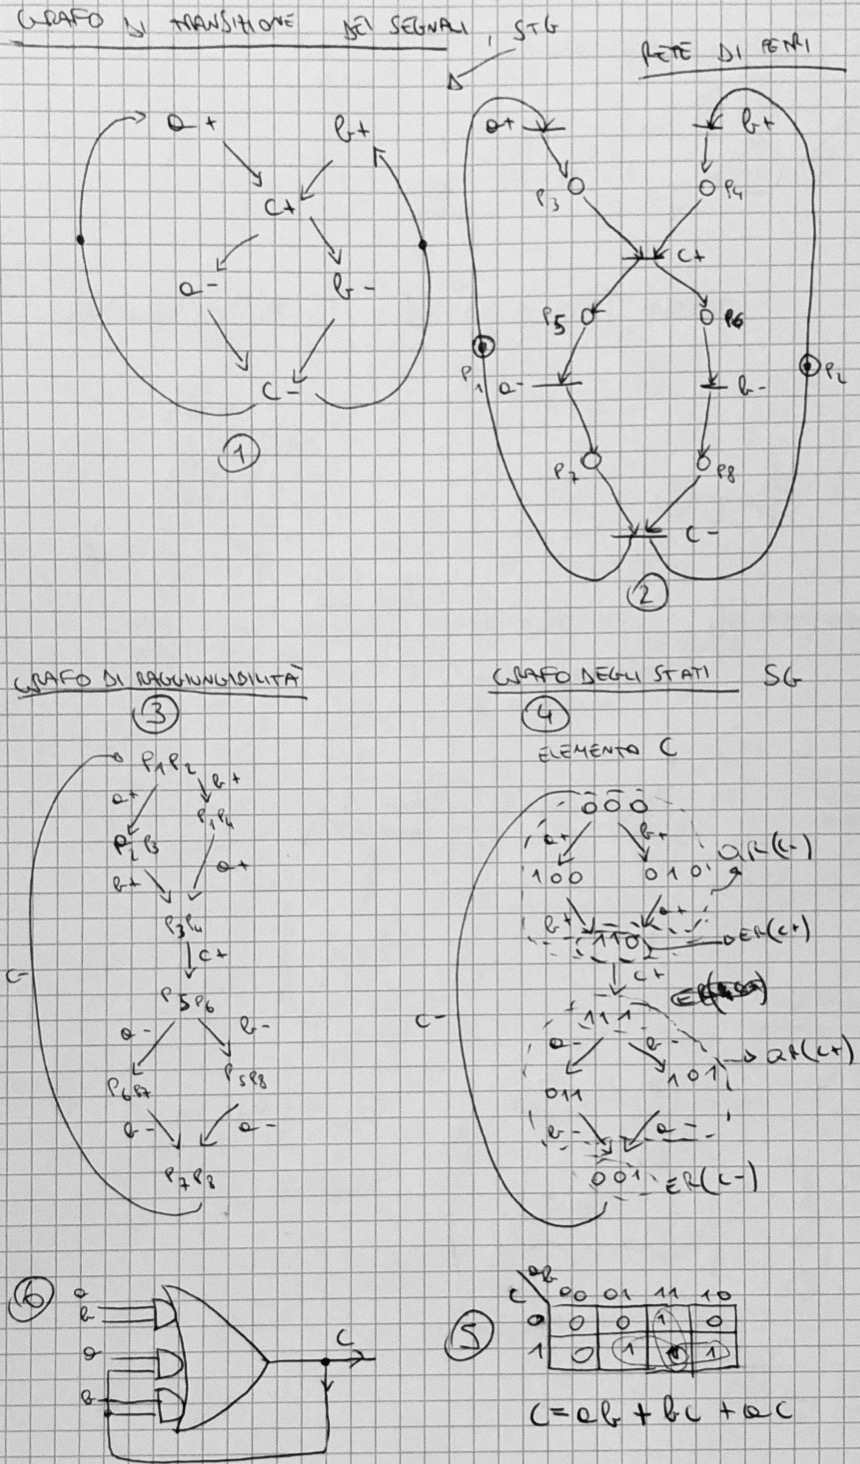
\includegraphics[scale=0.22]{macchinestati}
	\end{figure}
\end{multicols}

\subsection*{Determinizzazione di un NFA (Subset Construction)}
\addcontentsline{toc}{section}{Determinizzazione di un NFA (Subset Construction)}
Dato un automa \textit{NFA}, si può ottenere un automa \textit{output-deterministico} con il seguente algoritmo:
\begin{itemize}
	\item lo stato iniziale del DFA corrisponde a tutti gli stati iniziali dell'NFA;
	\item per ciascun stato componente prendo una alla volta le coppie (input/output) e genero i nuovi macrostati composti dai diversi stati target delle transizioni;
	\item ripetere il passo precedente fino a raggiungere un macrostato finale (contiene uno stato finale).
\end{itemize}
\begin{multicols}{2}
	\begin{figure}[H]
		\centering
		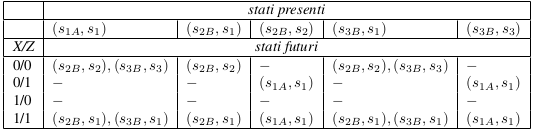
\includegraphics[scale=0.40]{DetNFA}
	\end{figure}
\columnbreak
\noindent
	Gli stati ($s_{2B}$, $s_2$) e ($s_{3B}$, $s_3$) sono equivalenti (le loro colonne di stati futuri coincidono). Perciò ci riduciamo a una tavola con una colonna in meno, dove lo stato ($s_{3B}$, $s_3$) è rimpiazzato dallo stato ($s_{2B}$, $s_2$).
\end{multicols}
\begin{multicols}{2}
\begin{figure}[H]
	\centering
	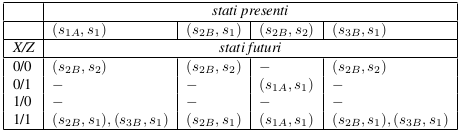
\includegraphics[scale=0.40]{DetNFA2}
\end{figure}
\columnbreak
\begin{multicols}{2}
	\noindent
	Gli stati ($s_{1A}$, $s_1$), ($s_{2B}$, $s_1$) e ($s_{3B}$, $s_1$) sono equivalenti (ci riduciamo a una tavola con due colonne in meno).
	\columnbreak
\begin{figure}[H]
	\centering
	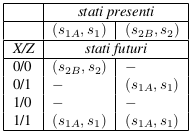
\includegraphics[scale=0.40]{DetNFA3}
\end{figure}
\end{multicols}
\end{multicols}


\subsection*{Minimizzazione}
\addcontentsline{toc}{section}{Minimizzazione}
\textbf{Input}: macchina a stati $M$.\\
\textbf{Output}: \textit{minimize($M$)}, cioè la macchina a stati con il minor numero di stati che sia bisimile a $M$ (il risultato è unico salvo rinominazione degli stati).\\
L'algoritmo si basa su due passi:
\begin{itemize}
	\item \textit{Output split}: in un set, se tutte le transizioni con un certo input hanno stesso output ok, se stesso input ma diverso output allora divido gli stati mettendoli in set diversi;
	\item \textit{Next-state split}: preso un set ottenuto, se ho degli stati che con uno stesso input raggiungono set diversi, allora faccio uno split.
\end{itemize}

\noindent
Ogni insieme di stati ottenuto rappresenta un singolo stato della macchina a stati bisimile a $M$.


\subsection*{Simulazione}
\addcontentsline{toc}{section}{Simulazione}
Date due macchine a stati $M_1$ e $M_2$, possiamo dire che $M_2$ simula $M_1$ se:
\begin{itemize}
	\item per ogni mossa di $M_1$, $M_2$ deve poter rispondere raggiungendo la stessa coppia (input/output);
	\item si aggiunge all'insieme della relazione di simulazione la coppia di stati raggiunti dalle due macchine.
\end{itemize}

\noindent
Ogni stato iniziale di $M_1$ è simulato da uno stato iniziale di $M_2$, e se uno stato $p$ di $M_1$ è simulato da uno stato $q$ di $M_2$, per ogni ingresso e per ogni stato futuro $p'$ di $p$ c’è uno stato futuro $q'$ di $q$ tali che $p'$ e $q'$ producono la medesima uscita e $p'$ è simulato da $q'$.

\subsection*{Bisimulazione}
\addcontentsline{toc}{section}{Bisimulazione}
Vale la bisimulazione se vale la simulazione in entrambi i versi (condizione necessaria ma non sufficiente). Se le relazioni di simulazione sono simmetriche, vale sicuramente la bisimulazione. Si testano le simulazioni in entrambi i versi scegliendo arbitrariamente quale macchina muoverà per prima ad ogni turno.
\newline

\noindent
La \textit{bisimulazione} tra $M_1$ e $M_2$ indica che gli stati iniziali delle due macchine sono in relazione e, per ogni stato $p$ di $M_1$, in relazione con $q$ di $M_2$, per ogni valore in input $p$ e $q$ producono lo stesso valore in output e gli stati successivi sono ancora in relazione.


\chapter*{Automi ibridi}
\addcontentsline{toc}{chapter}{Automi ibridi}
Si consideri una palla che rimbalza. Al tempo $t = 0$, la palla è fatta cadere da un’altezza di $y(0) = H$ metri con $\dot{y}(0) = 0  ~metri/sec$. Dopo cade liberamente seguendo la legge $\ddot{y}(t) = -g$, con $g = 10 ~m/sec^2$ costante di gravità. A un tempo successivo $t_1$, la palla colpisce il suolo con una velocità $\dot{y}(t_1) < 0$
metri al secondo e si produce un evento discreto rimbalzo. La collisione è inelastica e la palla rimbalza con velocità $\dot{y}(t) = -a\dot{y}(t_1)$, con $0 < a < 1$ costante. Poi la palla risale sino a una certa altezza e ricade di nuovo al suolo e così ripetutamente.
\begin{itemize}
	\item locazioni: {$l_1$}, dove $l_1$ è la locazione iniziale con condizioni iniziali $y(0) := H$, $\dot{y}(0) := 0$;
	\item dinamica della locazione $l_1 : \ddot{y}(t) = -g$;
	\item transizione da $l_1$ a $l_1$ : $A/rimbalzo$, $\dot{y}(t) := -a\dot{y}(t)$, dove $A = \{(y(t), \dot{y}(t)) | y(t) = 0\}$ (la sintassi delle annotazioni di una transizione è \textit{guardia/uscita}, \textit{azione});
	\item ingresso assente perché il sistema è autonomo;
	\item uscita $e_u(t) \in \{rimbalzo, assente\}$,\\
	uscita $y(t) \in \mathbb{R}$.
\end{itemize}
\begin{multicols}{2}
	\begin{figure}[H]
		\centering
		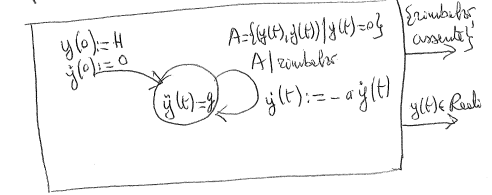
\includegraphics[scale=0.40, angle=-3.5]{SistemaIbrido}
	\end{figure}
	\begin{figure}[H]
		\centering
		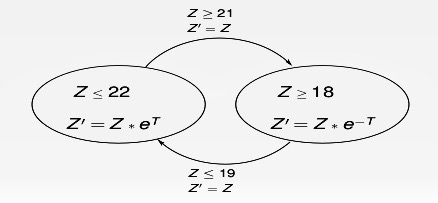
\includegraphics[scale=0.40]{Termostato}
		\captionsetup{labelformat=empty}
		\caption{Termostato}
	\end{figure}
	\columnbreak	
	\begin{figure}[H]
		\centering
		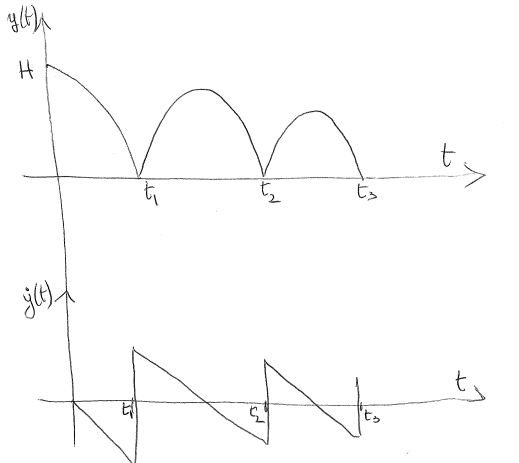
\includegraphics[scale=0.40, angle=-0.7]{Palla}
		\captionsetup{labelformat=empty}
		\caption{Grafico qualitativo}
	\end{figure}
\end{multicols}

\noindent
\textit{\textbf{Comportamento Zenoniano}}: numero infinito di transizioni discrete in un tempo finito.
\begin{figure}[H]
	\centering
	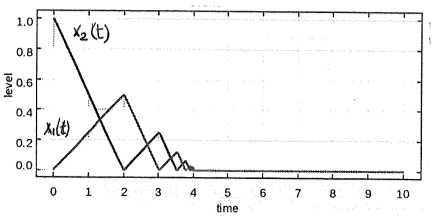
\includegraphics[scale=0.35]{Cisterne}
	\caption*{Esempio: cisterne}
\end{figure}



\chapter*{Definizioni}
\addcontentsline{toc}{chapter}{Definizioni}
\textit{\textbf{Macchina di Moore}}:\\L'uscita non dipende dall'ingresso, ma solo dallo stato corrente.
\\\\
\textit{\textbf{Macchina di Mealy}}:\\L'uscita è determinata dallo stato corrente e dall'ingresso corrente.
\\\\
\textit{\textbf{Supervisore}}:\\Se il sistema è sia controllabile che osservabile allora esiste il \textit{supervisore}.
\\\\
\textit{\textbf{Composizione Prodotto}}:\\$f ((x_1,x_2), \sigma) := (f_1(x_1,\sigma), f_2(x_2,\sigma))$ se $\sigma\in \Gamma_1 (x_1) \cap \Gamma_2(x_2)$
\\
Proprietà:\begin{itemize}
	\item $\Gamma_{1 \times 2} (x_1, x_2) = \Gamma_1 (x_1) \cap \Gamma_2(x_2)$
	\item $\mathcal{L} (G_ \times G_2) = \mathcal{L}(G_1) \cap \mathcal{L} (G_2)$
	\item $\mathcal{L}_m (G_ \times G_2) = \mathcal{L}_m(G_1) \cap \mathcal{L}_m (G_2)$
\end{itemize}
\noindent
\textit{\textbf{Composizione Parallela}}:\\
$f ((x_1,x_2), \sigma)  := 
\begin{cases}
(f_1(x_1,\sigma), f_2(x_2,\sigma)) &\text{ se } \sigma\in \Gamma_1 (x_1) \cap \Gamma_2(x_2) \\
(f_1(x_1,\sigma), x_2) & \text{ se } \sigma\in \Gamma_1 (x_1) \backslash E_2\\
(x_1, f_2(x_2,\sigma)) & \text{ se } \sigma\in \Gamma_2 (x_2) \backslash E_1
\end{cases}$
\\
Proprietà:\begin{itemize}
\item $\mathcal{L} (G_1 || G_2) = P^{-1}_1[\mathcal{L}(G_1)] \cap P^{-1}_2[\mathcal{L}(G_2)]$
\item $\mathcal{L}_m (G_1 || G_2) = P^{-1}_1[\mathcal{L}_m(G_1)] \cap P^{-1}_2[\mathcal{L}_m(G_2)]$
\end{itemize}

\noindent
\textit{\textbf{Controllabilità}}:\\
Siano $K$ e $M = \overline{M}$ linguaggi dell'alfabeto di eventi $E$, con $E_{uc} \subseteq E$. Si dice che $K$ è controllabile rispetto a $M$ e $E_{uc}$ se per tutte le stringhe $s \in \overline{K}$ e per tutti gli eventi $\sigma \in E_{uc}$ si ha: $s\sigma \in M \Rightarrow s \sigma \in \overline{K}$.\\Per la definizione di controllabilità si ha che $K$ è controllabile sse $\overline{K}$ è controllabile.
\\\\
\textit{\textbf{Macchina a stati deterministica}}:\\
Una macchina a stati è deterministica se esiste un solo stato iniziale. Inoltre per ogni stato e \textit{per ogni input} esiste solo uno stato successivo.
\\\\
\textit{\textbf{Non-Deterministico}}:\\
Per ogni segnale in input ci sono uno o più segnali in output, dunque questi sistemi hanno più \textit{behaviors}.
Può esserci più di uno stato iniziale e per ogni stato e ogni coppia di I/O può esserci più di uno stato successivo.
\\\\
\textit{\textbf{Output-Deterministico}}:\\
C'è solo uno stato iniziale e per ogni stato e per ogni coppia di I/O c'è solo uno stato successivo. Per ogni \textit{behavior} $(x,y)$ c'è una sola esecuzione. Per ogni macchina a stati non deterministica si può trovare una macchina a stati output-deterministica equivalente (attraverso la \textit{subset construction}).\\
Deterministico implica Output-Deterministico, ma non viceversa.

\noindent
\textit{\textbf{Non-Deterministico, Progressivo}}:\\
Significa che l'evoluzione è definita per ogni ingresso, cioè la funzione di transizione è definita come: $Stati \times Ingressi \rightarrow P(Stati \times uscite)\backslash \emptyset$, dove $P$ è l'insieme potenza e $\emptyset$ impone che sia progressiva.
\\\\
\textit{\textbf{Raffinamento}}:\\
Il sistema $S_1$ raffina il sistema $S_2$ sse con $Time[S_1] = Time[S_2]$ hanno stessi input e output ed inoltre $behaviors [S_1] \subseteq behaviors [S_2]$. $S_1$ è più dettagliato mentre $S_2$ è un'astrazione delle proprietà di $S_1$.
\\\\
\textit{\textbf{Equivalenza}}:\\
Due macchine a stati $M_1$ e $M_2$ sono equivalenti sse implementano lo stesso sistema (funzione di I/O), cioè $\forall x \in input$, $M_1(x) = M_2(x) \in output$.\\
Sono equivalenti se $behaviors [M_1] = behaviors [M_2]$.\\
Sono equivalenti sse esiste una bisimulazione tra $M_1 e M_2$. 
\\Sono equivalenti sse $M_1$ raffina $M_2$ e $M_2$ raffina $M_1$.
\\\\
\textit{\textbf{Simulazione - Raffinamento}}:\\
Se $M_2$ è deterministica, $M_1$ è simulata da $M_2$ sse $M_1$ raffina $M_2$ e $M_2$ raffina $M_1$.
\\
Se $M_2$ è pseudo-nondeterministica, $M_1$ è simulata da $M_2$ sse $M_1$ raffina $M_2$.
\\
Se $M_2$ è nondeterministica, $M_1$ è simulata da $M_2$ se $M_1$ raffina $M_2$ (ma $M_1$ raffina $M_2$ non implica che $M_1$ è simulata da $M_2$).
\\\\
\textit{\textbf{Linguaggi Normali}}: siano dati $M = \overline{M} \subseteq E^*$ e la proiezione $P$. Un linguaggio $K \subseteq M$ si dice \textit{normale} rispetto a $M$ e $P$ se: $ \overline{K} = P^{-1} [P(\overline{K})] \cap M $
\\\\
\textit{\textbf{Linguaggi Regolari - Reti di Petri}}:\\
I Linguaggi Regolari sono un sottoinsieme di quelli accettati dalle Reti di Petri.
\\\\
\textit{\textbf{Osservabilità e Intersezione}}:\\
L'osservabilità non è preservata dall'intersezione, dati $K_1$ e $K_2$ osservabili, $K_3 = K_1 \cap K_2$ non è osservabile.
Dato che l'intersezione non preserva l'osservabilità, non è garantita l'esistenza del sovralinguaggio osservabile infimo.
\\\\
\textit{\textbf{Osservabilità e Unione}}:\\
L'osservabilità non è preservata dall'unione, dati $K_1$ e $K_2$ osservabili, $K_3 = K_1 \cup K_2$ non è osservabile.
\\\\
\textit{\textbf{Rete di Petri Limitata}} (può non essere conservativa, ad esempio se ha un posto e una transizione):\\
È limitata se non ci sono $\omega$ nell'albero di copertura, quindi $k$ è il massimo numero di gettoni che possono accumularsi in un posto, e non $\infty$.\\
Un posto è limitato se $\exists k \geq 0$ tale che, per ogni marcatura raggiungibile, il numero di gettoni del posto $\leq k$. Una rete è limitata se ogni posto è limitato.
\\
\textit{\textbf{Rete di Petri Viva}}:\\
Una rete di Petri con marcatura iniziale $x_0$ è viva se da ogni transizione $t$ e da ogni marcatura $x_M$ raggiungibile da $x_0$ esiste una marcatura $x_t$ raggiungibile da $x_M$ dove $t$ è abilitata a scattare. Cioè se da ogni nodo dell'albero si può far scattare qualsiasi transizione (da ogni marcatura si può ritornare alla marcatura iniziale e da lì far scattare qualsiasi transizione).
\\
\textit{\textbf{Rete di Petri Conservativa}} (dunque anche limitata):\\
Il numero di token nella rete è costante, cioè $\sum_{i=1}^{b} \gamma_i x(p_i) = C$ dove $b$ sono i posti limitati (senza mai $\omega$).\\
\MakeUppercase{è} \textit{strettamente conservativa} se per ogni marcatura raggiungibile, è invariata la somma dei gettoni.\\
Una rete è conservativa se esiste un vettore di interi tale che, per ogni marcatura raggiungibile, è invariata la somma pesata dei gettoni nei posti.
\\
\textit{\textbf{Rete di Petri Reversibile}} (se il suo grafo di raggiungibilità è fortemente connesso):\\
È reversibile se da ogni marcatura raggiungibile è possibile ritornare alla marcatura iniziale.
\\\\
\textit{\textbf{Rete di Petri Ordinaria}}: è ordinaria se tutti gli archi anno peso unitario.
\\
\textit{\textbf{Rete di Petri Pura}}: è pura se non contiene cappi.
\\
\textit{\textbf{Rete di Petri Ristretta}}: è ristretta se è ordinaria e pura.
\end{document}